\chapter{Methods}
\section{Data}\label{data}

\subsection{Dataset}

The dataset for this research comes from the Massachusetts Bay Transportation Authority (MBTA).  The data is publicly available and consists of the following

\begin{itemize}
  \item GPS data for buses, consisting of latitude, longitude, route, and route direction
  \item Route data, describing the GPS location of stops along a route
  \item Bus timetable information, which shows the times when a bus arrives at each stop in a route
  \item Bus metadata
\end{itemize}

Buses, routes and stops are described by ids.  Bus stops also have human readable names indicating their location.
The dataset spans several years, and includes all of the buses and routes in Boston.
This dataset is unique from previous research in its extent both in size and duration.
Previous studies use several months of data, whereas this dataset allows the analysis of longer term trends, including seasonal trends.

Figure~\ref{gps} shows GPS data for Route 1.  The route starts in Cambridge at Massachusetts Avenue and Holyoke Street, and ends in Boston at Dudley Station.
The GPS data is fairly accurate for the most part.
However, in cities like Boston, GPS data suffers from an issue known as urban canyons.
This occurs on relatively narrow streets with very tall skyscrapers, where a canyon effect is created.
The large buildings obscure satellite signals, creating very noisy GPS signals.
Certain streets in Boston suffer from this issue, however Route 1 does not touch those streets, results in relatively clean GPS data.
All of the data points are well localized to the street.

\begin{figure}
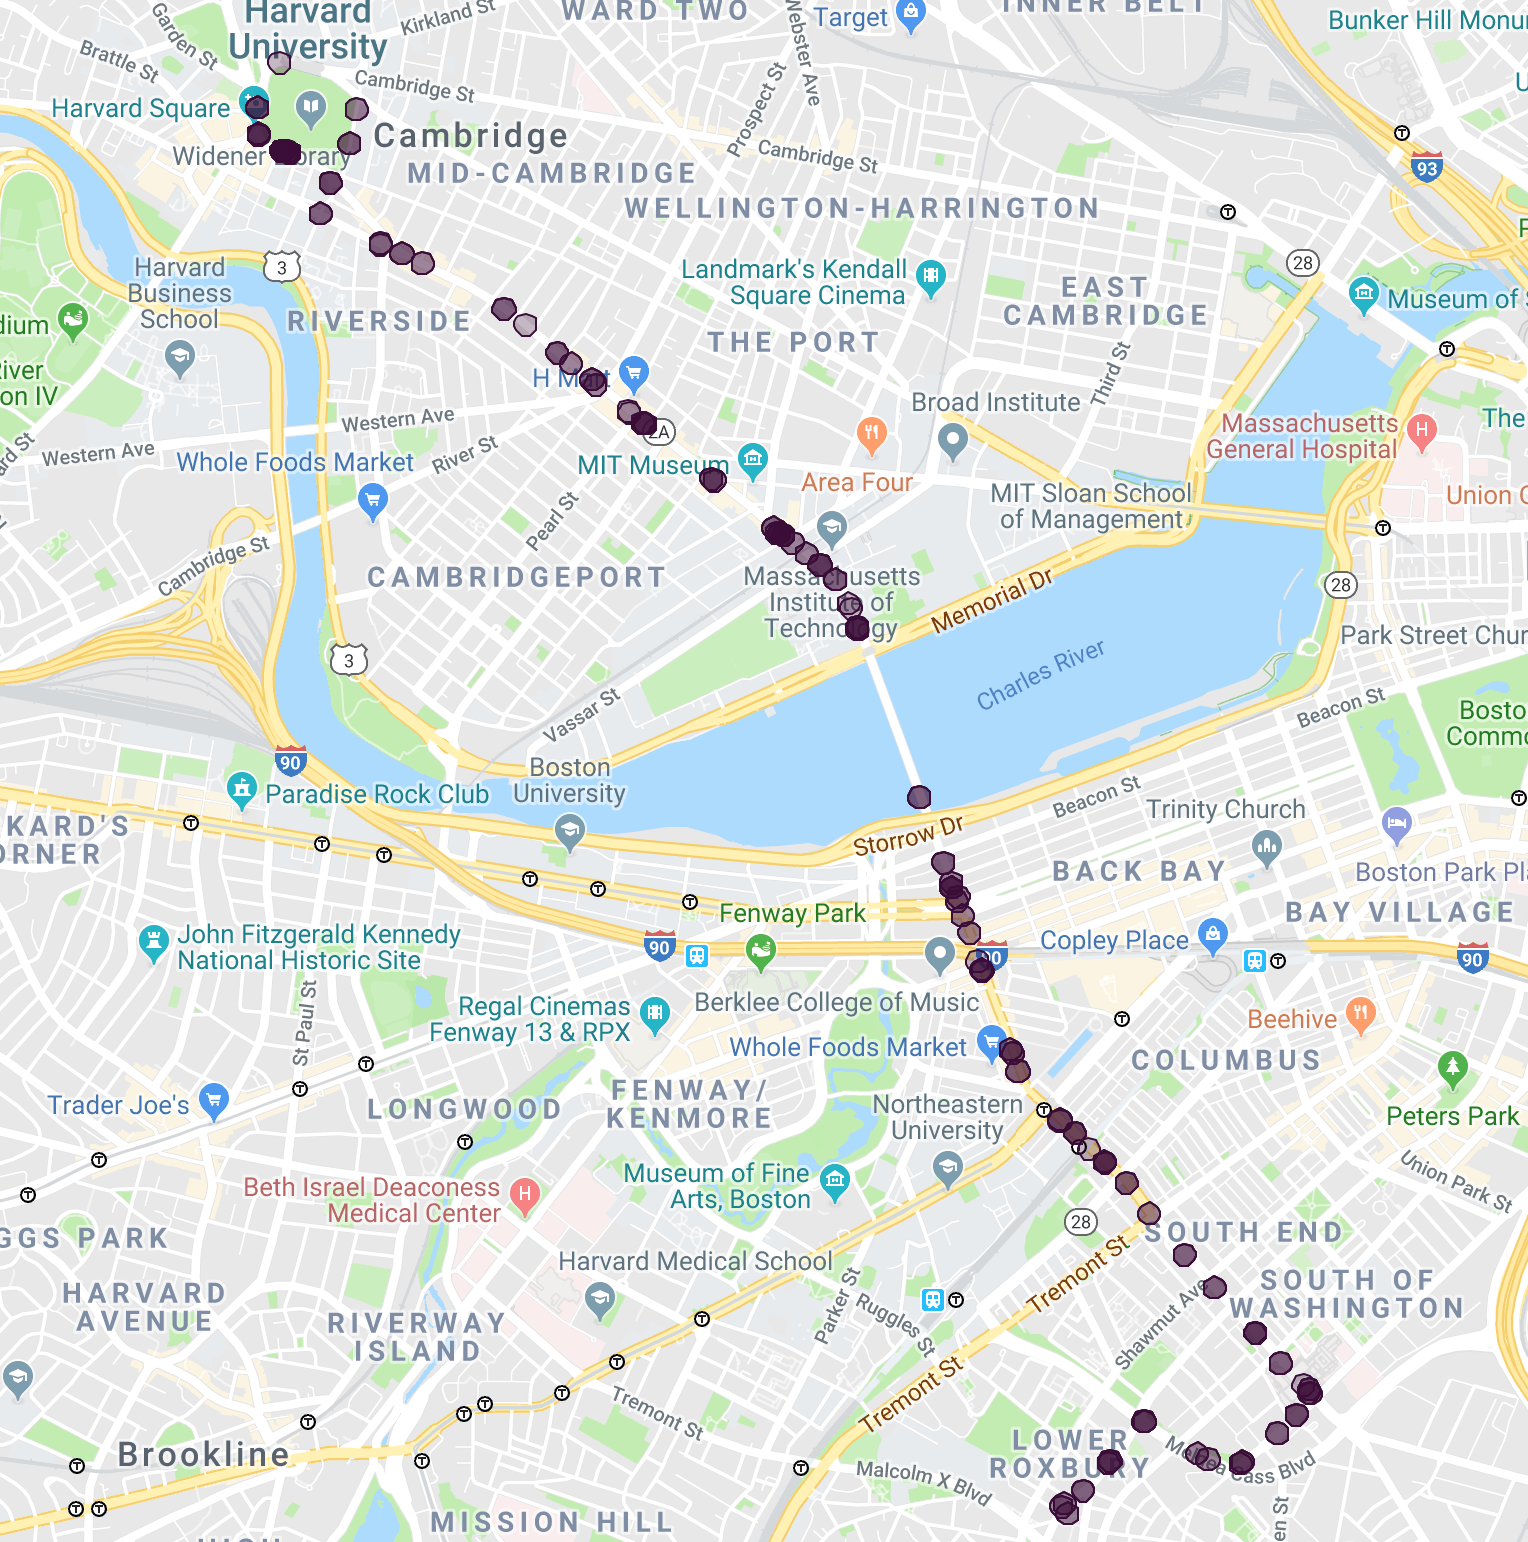
\includegraphics[width=\linewidth]{images/map.png}
%\vspace{2.4in}
\caption{GPS Data from Route 1 serving Cambridge and West Boston}
\label{gps}
\end{figure}

\subsection{Interpolating Trajectories}

The data provided consists of tuples of latitude, longitude, bus id, and timestamp.
However, the data needed to train the model involves the arrival times at each stop, so the trajectory of the bus must be interpolated from the noisy GPS data.
This is done via the following process

\begin{enumerate}}
\item Tuples are grouped by bus id and route, then sorted in time
\item The GPS trajectory is then converted from latitude and longitude into a 2D Cartesian projection
\item The entire trajectory of the bus is segmented into each individual trip along the route
\item The 2D coordinates are then projected onto the route using a Gaussian noise assumption, shown in Figure~\ref{path}
\item This (x,y,t) data is the converted from a 2D position on the map to a 1D distance along the route, because all buses follow the same route
\item Stop data of the form (latitude, longitude) is then converted into the same 1D distance along the path.
\item The trajectory of the bus is then interpolated in a piecewise linear fashion, assuming a constant speed between adjacent points.
\item The trajectory is sanitized by removing any erroneous data by thresholding the velocity of the vehicle
\item This trajectory can then be used to determine the arrival time at each stop by determining the timestep when each bus was within a certain threshold of the stop. This is illustrated in Figure~\ref{interpolate}.
\end{enumerate}}

\begin{figure}
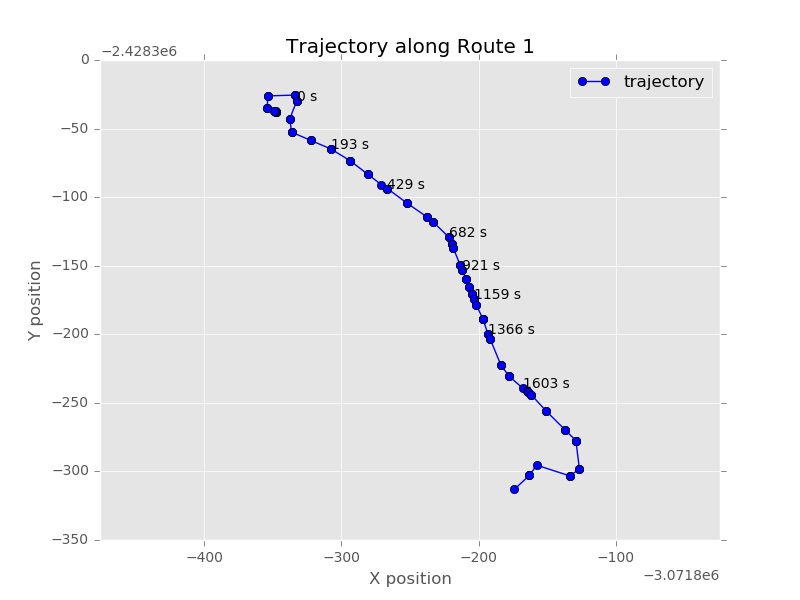
\includegraphics[width=\linewidth]{images/path.png}
%\vspace{2.4in}
\caption{(x,y,t) trajectory of bus along route 1. The routes starts on the top left and finishes on the bottom right.}
\label{path}
\end{figure}

\begin{figure}
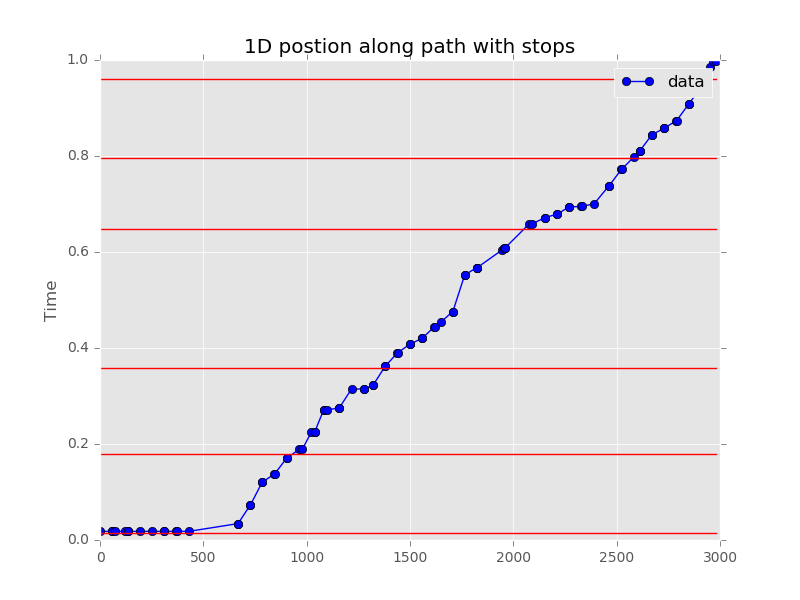
\includegraphics[width=\linewidth]{images/interpolate.png}
%\vspace{2.4in}
\caption{Interpolated trajectory of bus (blue) with stop locations overlain (red). Intersections indicate the bus arriving at a stop.}
\label{interpolate}
\end{figure}

\subsection{Features}

The following are a number of features which are commonly used as variables to model bus networks.

\begin{itemize}
  \item Arrival Time: Time the bus arrives at a stop
  \item Travel Time: The difference in arrival times between two stops
  \item Dwell Time: The amount of time a bus spends at a stop
  \item Schedule Adherence: The difference between the projected arrival time and the actual arrival time
  \item Headway: The difference in arrival time for two adjacent buses at a specific stop
  \item Direction: For a route which runs in both directions
  \item Weather
  \item Traffic Congestion
  \item Day of Week
  \item Month of Year
\end{itemize}

The arrival time at each stop is computed as shown above.
Travel time can them be trivially computed by taking the difference between two arrival times.
Schedule adherence is computed by comparing the arrival time of the bus the closest listed arrival time.
Other features are either derived from the raw data or pulled from outside sources.

\subsection{Distribution of Arrival Times}

Figure~\ref{dist} is a histogram of the difference in arrival times between adjacent buses at a particular stop on Route 1.
Three plots are overlain on the distribution.
If the buses ran perfectly on schedule, the distribution should be concentrated about the mean, indicated by the dotted black line.
If the buses are perfectly random and independent, the distribution should follow a Poisson distribution.
However buses are not independent.
In particular, a bus will not pass another bus, which leads to the high concentration about zero in the distribution.
This effect is compounded bus clumping.
This effect is well captured by an exponential distribution.
More complicated distribution like the GUE have been used to describe intervals between buses.
A study out of Cuernavaca, Mexico \cite{baik2006model} first identified this effect, and the same effect is observed in the New York public transit system.

\begin{figure}
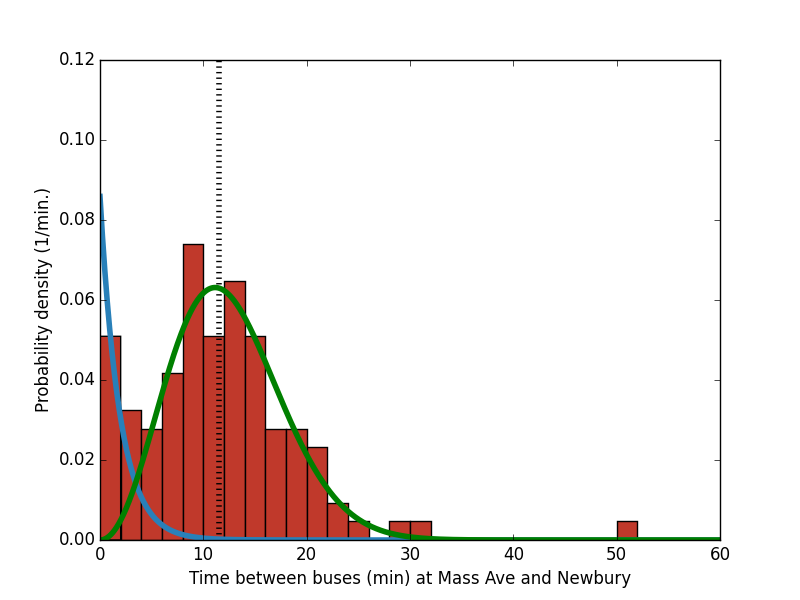
\includegraphics[width=\linewidth]{images/dist.png}
%\vspace{2.4in}
\caption{Distribution of intervals between bus arrival times at Newbury and Mass. Ave.}
\label{dist}
\end{figure}

\section{Models}\label{models}
\subsection{Linear}
\subsection{Multilayer Perceptron}
\subsection{Convolutional Neural Network}
\subsection{Recurrent Neural Network}
\section{Training}\label{training}
\section{Inference}\label{inference}
